\documentclass[addpoints]{exam}
\usepackage[utf8]{inputenc}
\usepackage{xcolor}
\definecolor{light-gray}{gray}{0.95}
\newcommand{\code}[1]{\colorbox{light-gray}{\texttt{#1}}}

\usepackage{hyperref}
\hypersetup{
    colorlinks=true,
    linkcolor=blue,
    filecolor=magenta,      
    urlcolor=blue,
}
\usepackage{tikz,lipsum,lmodern}
\usepackage[most]{tcolorbox}
\usepackage{url}


%This block of commented code translates default words to Spanish
%-------------------------------------------------------------
%\pointpoints{punto}{puntos}
%\bonuspointpoints{punto extra}{puntos extra}

%\totalformat{Pregunta \thequestion: \totalpoints{} puntos}

%\chqword{Pregunta}
%\chpgword{Página}
%\chpword{Puntos}
%\chbpword{Puntos extra}
%\chsword{Puntos obtenidos}
%\chtword{Total}

%\boxedpoints
%-------------------------------------------------------------

\begin{document}
%This code creates the text before the first question
%-------------------------------------------------------------------
\begin{center}
\fbox{\fbox{\parbox{5.5in}{\centering
Experimenting with Dynamic networks}}}
\end{center}

% \vspace{5mm}
% \begin{tcolorbox}[colback=black!5!white,colframe=white!75!black]
% You can do the exercises in the order that you prefer. \\  
% the \textit{Going further} experiments take more time and I do not expect everyone to do them.
% \end{tcolorbox}
% \vspace{5mm}

%Here, the questions begin


\begin{tcolorbox}[colback=black!5!white,colframe=white!75!black]
Several libraries exist to manipulate temporal networks, but most of them are not fully mature. I propose to use \code{tnetwork}, that can be installed using \code{pip}. 

Documentation and examples: \url{https://tnetwork.readthedocs.io}.

\end{tcolorbox}


\begin{questions}


\question Paths in dynamic networks

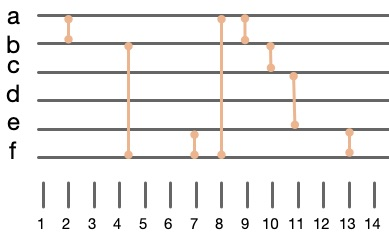
\includegraphics[width=0.5\textwidth]{pics/exo.jpg}

\begin{parts}
\part What is/are the \textbf{shortest} path from (a,1) to (e,14)?
\part What is/are the \textbf{foremost} path from (a,1) to (e,14)?
\part What is/are the \textbf{fastest} path from (a,1) to (e,14)?

\end{parts}

\question Characterizing a dynamic network as a sequence of snapshots

\begin{parts}
\part Using \code{tnetwork}, load the dynamic network of interactions between people in a hospital, collected by the sociopatterns project as a sequence of snapshots. (1 snapshot=20s, analysis over a few days)

You can do this with: \code{g = tn.graph\_socioPatterns\_Hospital(format=tn.DynGraphSN)}

\begin{tcolorbox}[colback=black!5!white,colframe=white!75!black]
You can read about this dataset and other information about the sociopatterns project on the following page: \url{http://www.sociopatterns.org/datasets/primary-school-temporal-network-data}

\end{tcolorbox}


\part Count the number of snapshots. You can obtain the list of times at which snapshots occur with \code{g.snapshots\_timesteps()}.

\part Obtain the graph corresponding to the first snapshot. You can use the \code{g.snapshots()} method which return a sorted dictionary, in which keys are times of snapshots and values are snapshots represented by a \code{networkx} graph object.

\part Compute the number of nodes and edges in this snapshot, and plot it.

\part What is the total number of interactions among all nodes at all time (edge-time)? What is the total number of different nodes? (you can use a \code{for} loop, and \code{set} or \code{collections.Counter} to handle repeated elements.

\part Plot the evolution of the number of nodes, number of edges and density along time. Plot the evolution of the degree of one particular node. Would you say that this network is rather stable or unstable? 

\part You can plot several graphs simultaneously using the following function:

\code{graph = tn.plot\_as\_graph(g,ts=[1254386420,1254386440,1254386460])}, with ts being a list of timestamps.

\part You can plot the presence of nodes in snapshots with the \code{tn.plot\_longitudinal(g,to\_datetime=True)}. The \code{to\_datetime} parameter allows to transform datetime to their corresponding date. Be careful, it might take about 30s on the full graph.

\part Compute the aggregated graph using \code{g.cumulated\_graph()}. Plot this graph, compute its number of nodes, edges, density. 

\part Compute snapshots aggregating activity every hour using \code{g2 =g.aggregate\_time\_period("hour")}. Analyze the resulting network in a way similar to the first graph. Do you think that this network is stable or unstable?


\part Compute (you have to write the code yourself) the dynamic version of "number/quantity" of nodes $N$, "number/quantity" of edges $L$ and density $d$ for the whole period, then for one particular day. You will have to use a \code{for} loop over all snapshots.
\end{parts}    





\vspace{5mm}
\question Going further: \textbf{Dynamic Communities}
\begin{parts}

\part Read the documentation of \code{tnetwork} about the detection of dynamic communities: \url{https://tnetwork.readthedocs.io/en/latest/notebooks/demo_DCD.html}. 
\part Apply several methods on the primary school dynamic network aggregated every hour and compare the results. (\code{tnetwork.graph\_socioPatterns\_Primary\_School(format=tn.DynGraphSN)}

\part Compute communities on the graph in its original form (no aggregation). Compute static communities on the cumulated graph (aggregated over the whole period). What do you think of the communities found using those three different approaches?

\end{parts}




\end{questions}


\end{document}